\chapter{Bread types}%
\label{ch:bread-types}
\begin{quoting}
In this chapter you will learn about different bread types and their
advantages and disadvantages.  You can also find very simple recipes for
flatbread and pan loaf.  The former is probably the most accessible, least
effort type of bread you can make, while the latter is a little more involved.
Free standing bread has its own chapter, due to its increased complexity.
\end{quoting}

\section{Introduction}%
\label{sec:intro}

In this section we classify bread by its baking techniques. The appearance and
taste will of course be different, but you can get excellent bread with each
of them. Some breads will require investment and technique, as depicted in
Table~\ref{tab:bread-types-comparison}.  Flatbread is probably the most
accessible, least effort type of bread you can make. If you are a busy person
and/or don’t have an oven, this might be exactly the type of bread you should
consider. 
\begin{table}[!htb]
    \begin{center}
        \documentclass[tikz]{standalone}
\usepackage{tikz}
\usepackage{siunitx}
\DeclareSIUnit\degF{\text{°}F}

\begin{document}
\begin{tabular}{|l|l|l|l|}
\hline
                                 & \textbf{Flat bread} & \textbf{Loaf pan bread} & \textbf{Free standing bread} \\ \hline
\textbf{Cooking method}          & Fire, pan, barbecue & Oven                    & Oven                         \\ \hline
\textbf{Working time in minutes} & 3                   & 5                       & 60                           \\ \hline
\textbf{Flour types}             & All                 & All                     & Gluten flours                \\ \hline
\textbf{Difficulty}              & Very easy           & Easy                    & Difficult                    \\ \hline
\textbf{Cost}                    & Low                 & Medium                  & High                         \\ \hline
\end{tabular}
\end{document}

        \caption[Different bread types]{An overview of different bread types
            and their respective complexity.}%
        \label{tab:bread-types-comparison}
    \end{center}
\end{table}

\section{Flatbread}%
\label{sec:flatbread}

Flatbread is probably the simplest sourdough bread to make.
To make a flatbread no oven is required; all you need is a stove.

\begin{figure}[!htb]
  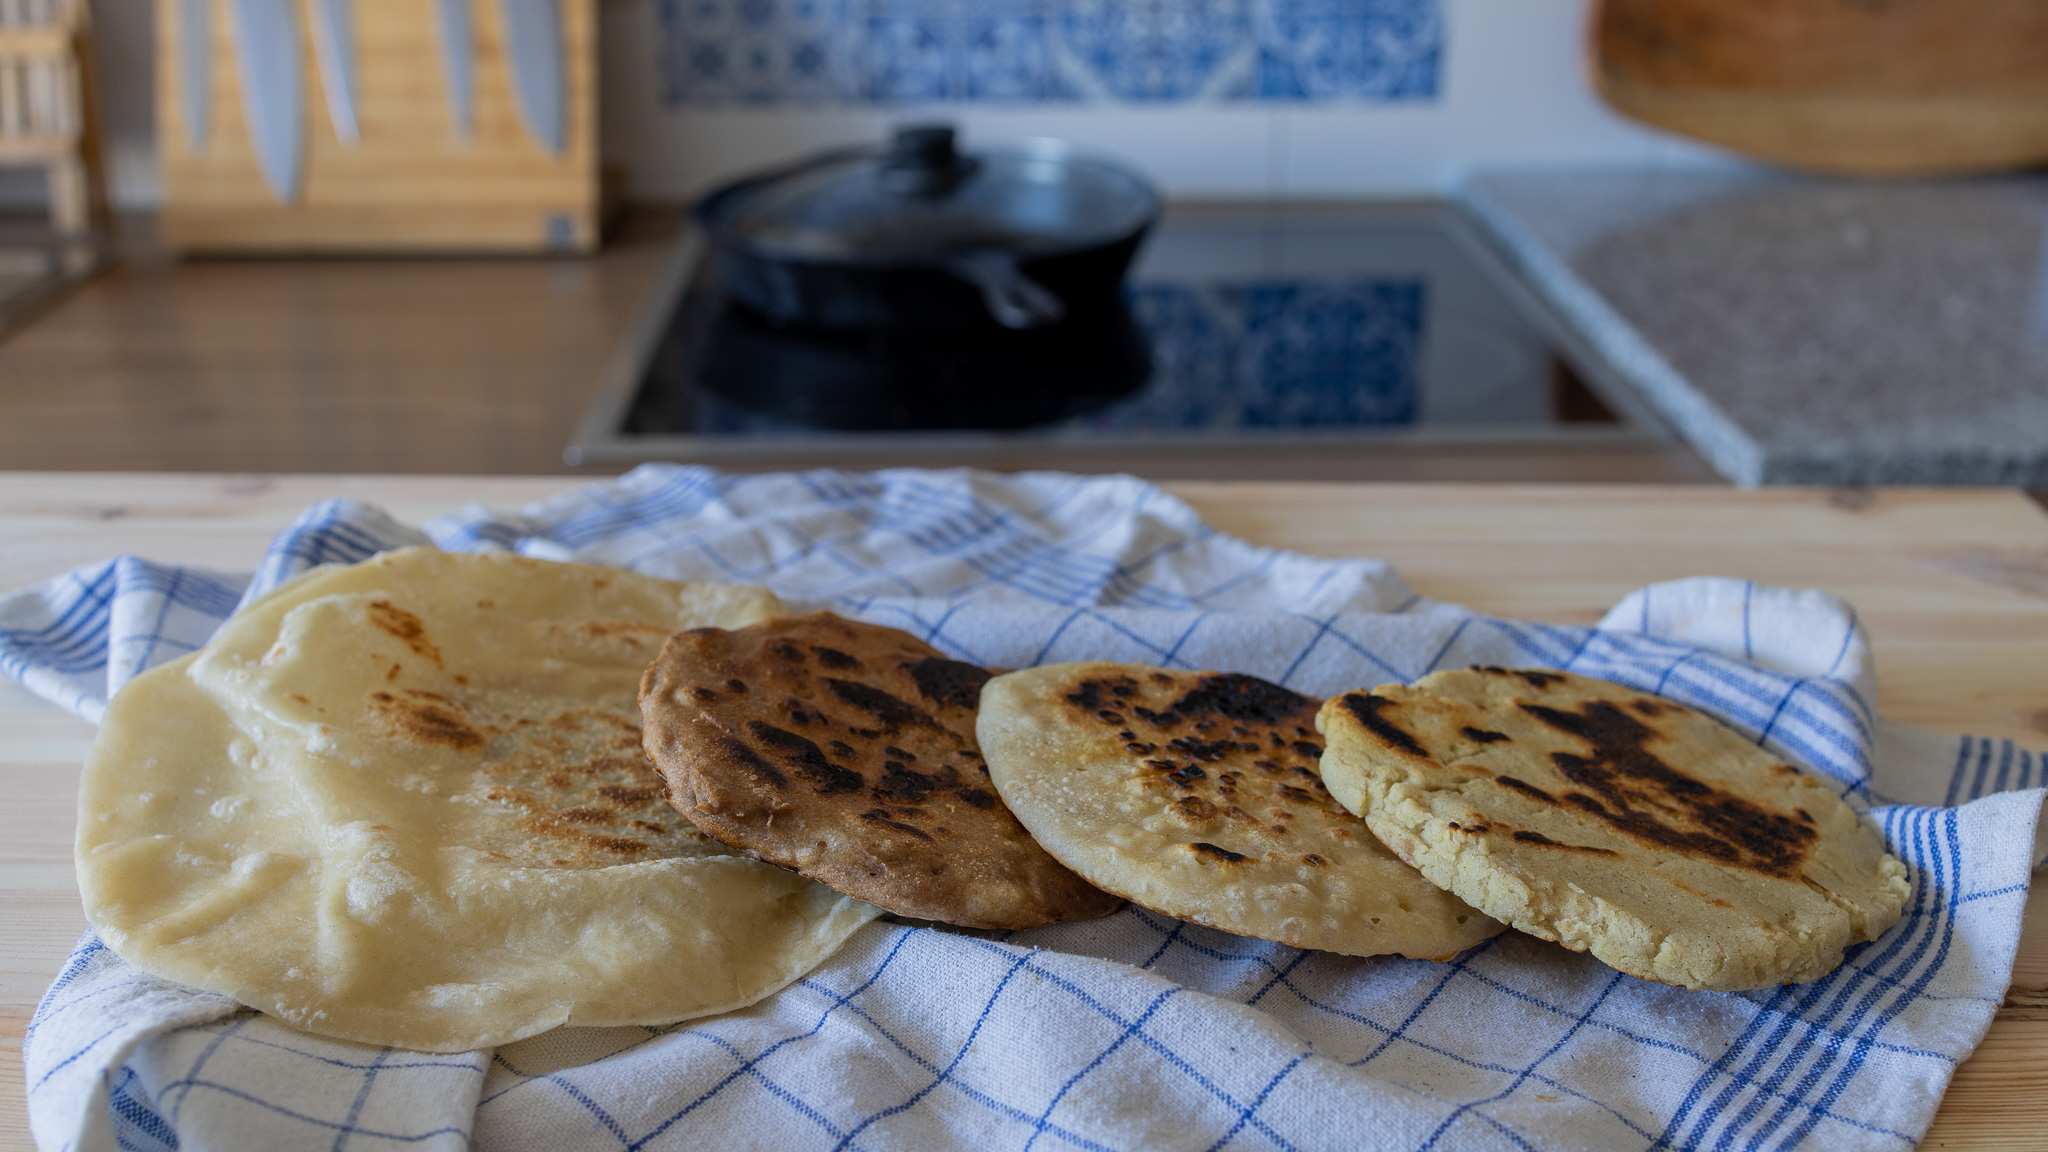
\includegraphics[width=\textwidth]{flat-breads-selection}
  \caption[Flatbread selection with different flours]{An assorted selection of
      different flatbreads made with sourdough. From left to right:
      Wheat~tortilla, rye, spelt and corn.}%
\end{figure}

This type of bread is super simple to make as you can skip
a lot of the technique that is normally required to make wheat doughs.
The flatbread can be made with all kinds of flours. You can even use
flour without gluten, such as corn or rice flour, to make the
dough. To make the flatbread a little more fluffy, you
can use a little bit of wheat flour. The developing gluten
will trap the gases. During baking, these gases will
inflate the dough.

Another trick to improve the texture of the flatbread is to
make a very wet dough. A lot of the water will evaporate
during the baking process and thus make the bread fluffier.
If your water content is very high, it will produce a
pancake-like consistency, as you can see in
Table~\ref{tab:flat-bread-ingredients}

\begin{table}[!htb]
    \begin{center}
        %TODO: last line is not great
\begin{tabular}{@{}>{\bfseries} p{0.15\textwidth}rlrl@{}}
\toprule
      & \multicolumn{2}{c}{\thead{Flat breads}} & \multicolumn{2}{c}{\thead{Pancakes}} \\ \midrule
Flour             & 100g   &           & 100g   &           \\ 
Water             & 100g   & (100\%)   & 300g   & (300\%)   \\ 
Sourdough starter & 5--20g & (5--20\%) & 5--20g & (5--20\%) \\ 
Salt              & 2g     & (2\%)     & 2g     & (2\%)     \\ 
Bake when?        & \multicolumn{2}{c}{Dough increased by 50\% in size.}
                  & \multicolumn{2}{c}{Bubbles visible on surface.}\\
\bottomrule
\end{tabular}

        \caption[Flatbread recipe]{Flatbread or pancake recipe for 1 person.
            Multiply the ingredients to increase portion size.  Refer to the
            Section~\ref{section:bakers-math}
            ``\nameref{section:bakers-math}'' to learn how to understand and
            use the percentages properly.}%
            \label{tab:flat-bread-ingredients}
    \end{center}
\end{table}

For a full recipe including the process of making such a flatbread,   refer to
Subsection~\ref{subsec:flat-bread-recipe}

\subsection{Flatbread framework}%
\label{subsec:flat-bread-framework}

As explained above, if you are just getting started, making a flatbread is the
easiest way to start making great bread at home. With just a
few steps, you can stop buying bread forever. This works with
any flour, including gluten-free options.

\begin{flowchart}[!htb]
\begin{center}
  \begin{tikzpicture}[node distance = 3cm, auto, every node/.style={inner sep=10, outer sep=0}]
\node [block] (init) {Mix ingredients};
  \node [block, right of=init, node distance=5cm] (wait) {Wait for dough to be ready};
  \node [block, right of=wait, node distance=5cm] (bake_bread) {Bake bread on stove};
  \path [line] (init) -- (wait);
  \path [line] (wait) -- (bake_bread);
\end{tikzpicture}

  \caption[The process to make a sourdough flatbread]{The process of making a flatbread is very
      simple, requiring very little effort. This type of bread is especially
      handy for busy bakers.}%
  \label{fig:flat-bread-process}
\end{center}
\end{flowchart}

This is my go-to recipe that I~use to make bread whenever
I~have little time or when I~am abroad. You can choose
between two options:
%
\begin{enumerate}
    \item A flatbread similar to a roti or naan bread
    \item Sourdough pancakes.
\end{enumerate}

To get started prepare your sourdough starter. If it has not been used for a very
long time, consider giving it another feed. To do so, simply take \qty{1}{\gram} of your
existing sourdough starter and feed it with \qty{5}{\gram} of flour and \qty{5}{\gram} of water.
If you do this in the morning, your sourdough starter will be ready in the evening. The
warmer it is, the sooner it will be ready,  consider
using warm water if it is very cold where you live.

\begin{figure}[htb!]
\begin{center}
  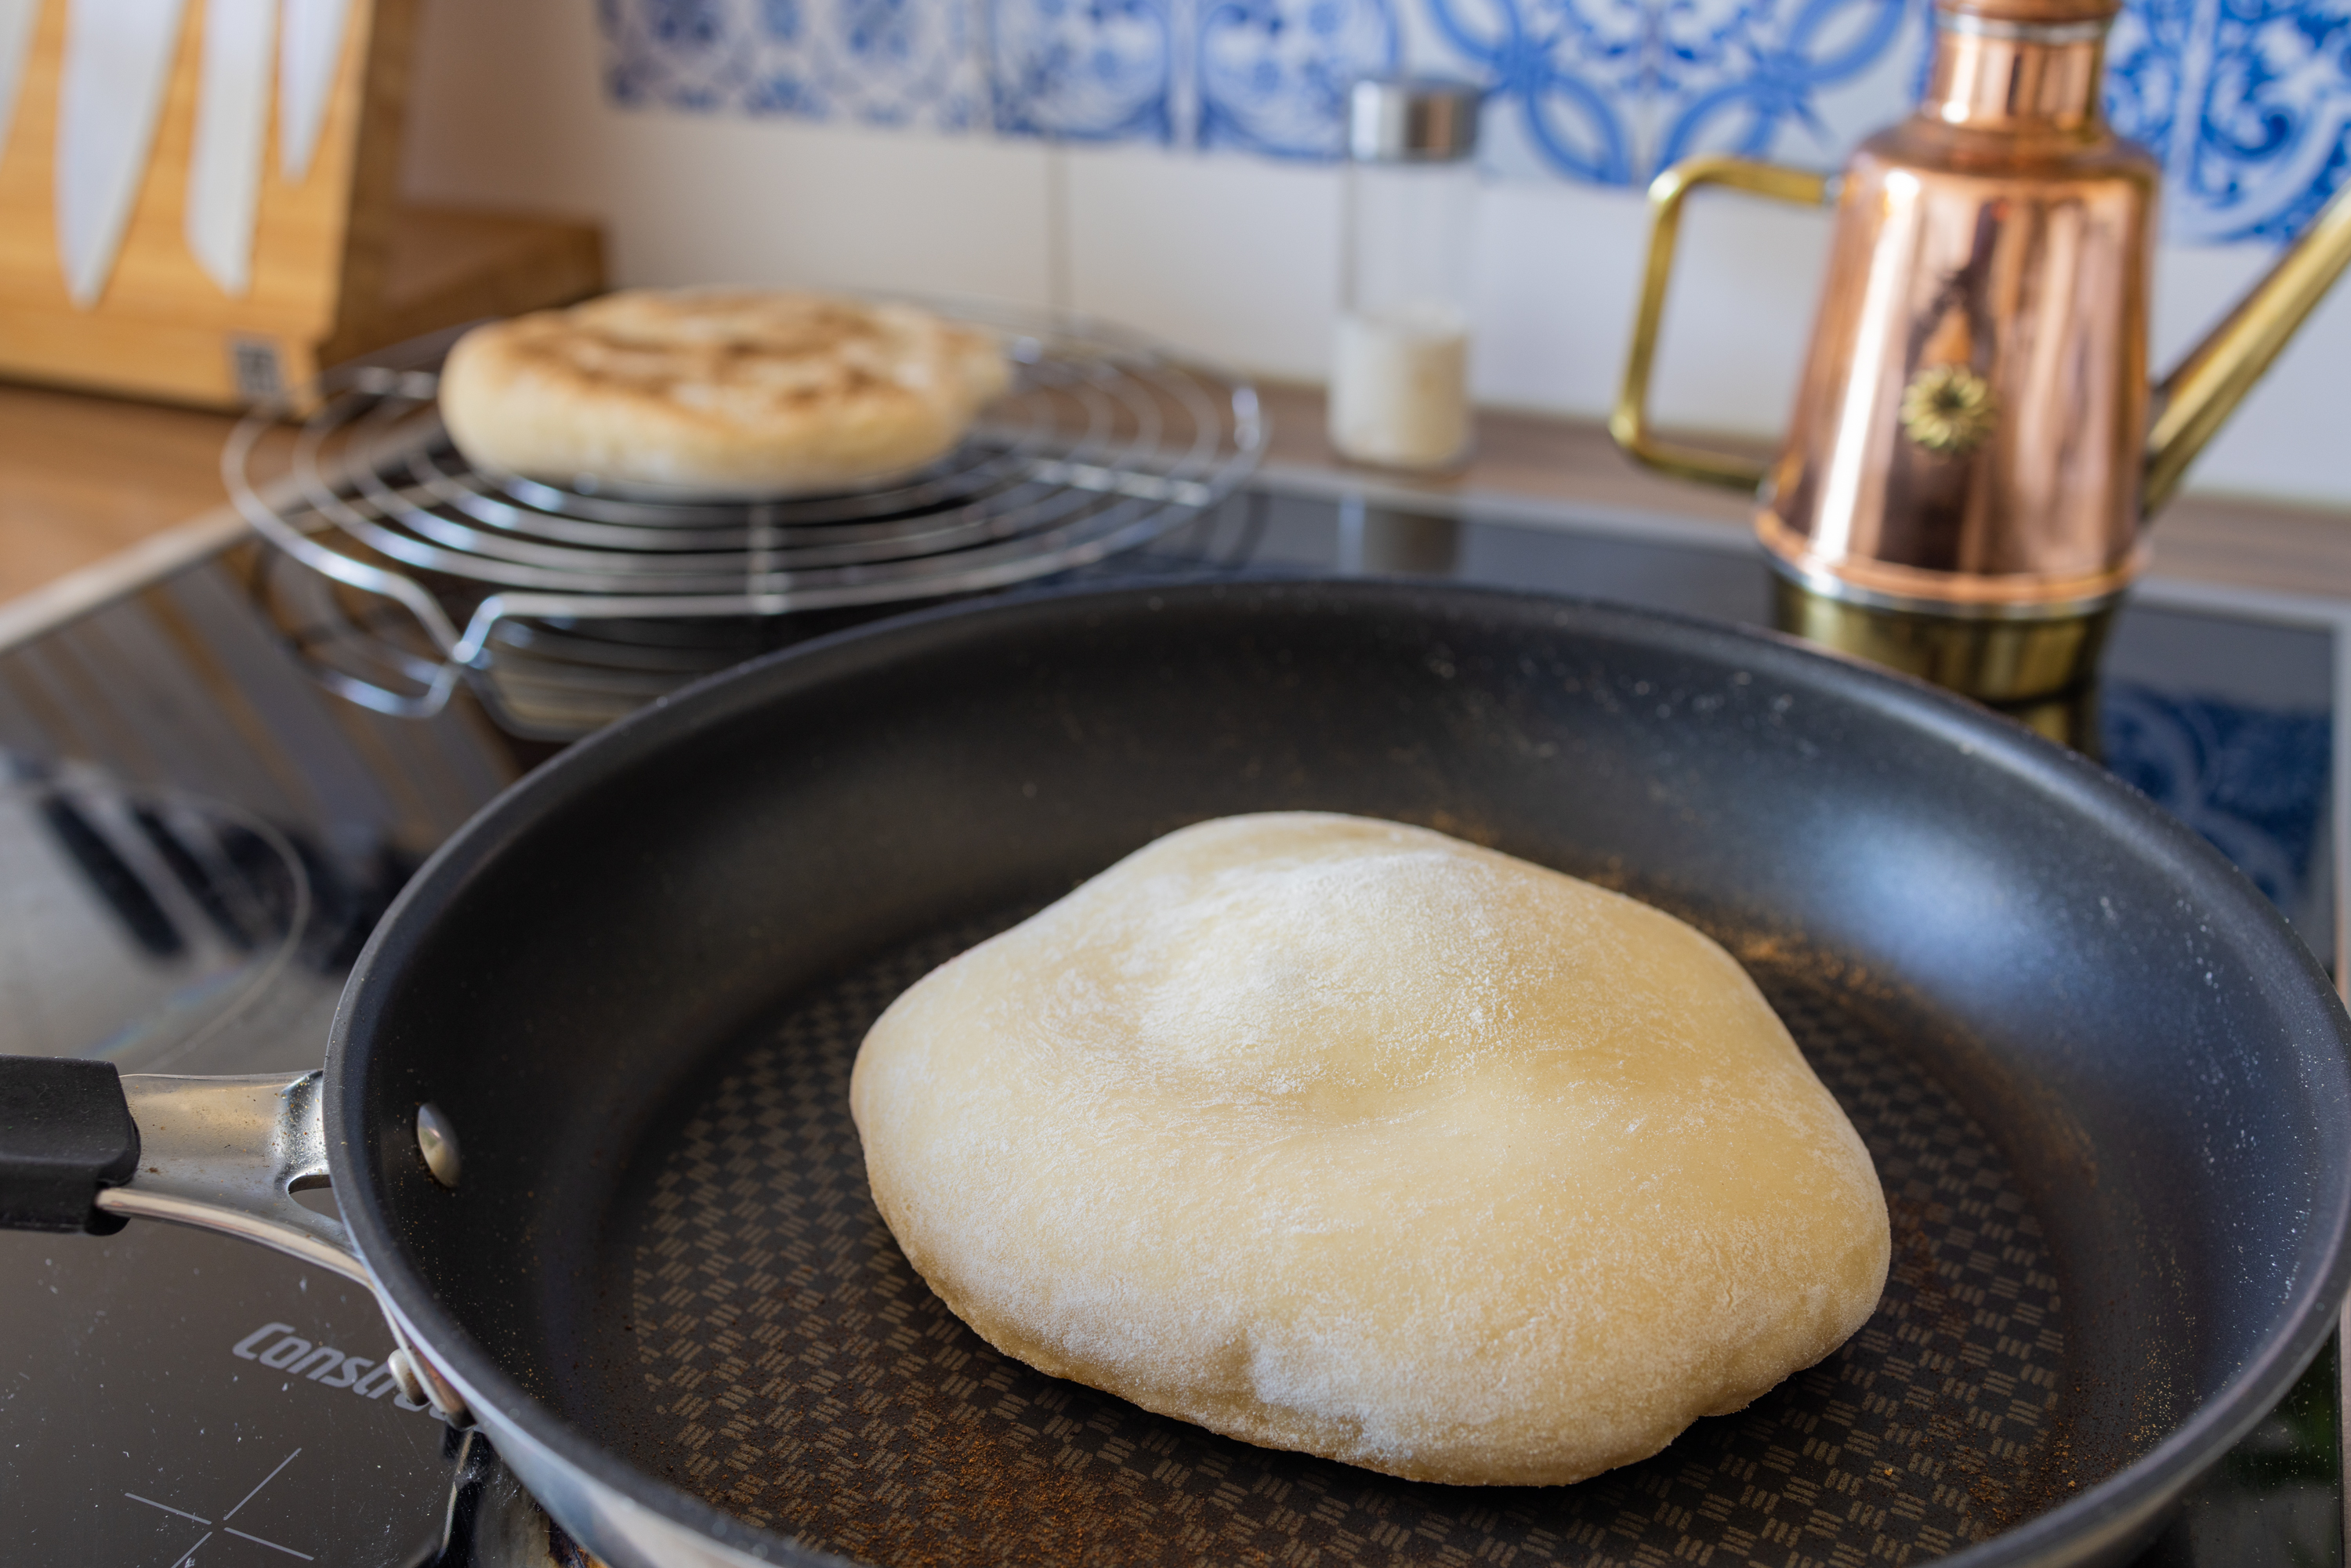
\includegraphics[width=1.0\textwidth]{flat-bread-wheat}
  \caption[Wheat flatbread]{A flatbread made with purely wheat flour. The
      dough is drier at around \qty{60}{\percent} hydration. The drier dough
      is a little harder to mix. As wheat contains more gluten, the dough
      puffs up during the baking process.}
\end{center}
\end{figure}

This way you should have around \qty{11}{\gram} of sourdough ready in the evening. You will have
the perfect quantity to make a dough for one person. In case you want to make more
bread, simply multiply the quantities shown in
Table~\ref{tab:flat-bread-ingredients}.

Then in the evening simply mix the ingredients as shown in the table. Your dough
is going to be ready in the morning. It's typically ready after 6--12~hours. If
you use more sourdough starter it will be ready faster, conversely it will take
longer if you use less. Try to aim for a fermentation time of 8--12~hours as
by using your dough too soon, the flavor might not be as good. By using your
dough later it might become a little more sour. The best option is to
experiment and see what you personally like the most.

After mixing the ingredients together cover the container, this prevents the
dough from drying out and makes
sure no fruit flies get access. A transparent container will be helpful
when getting started. You can observe the dough more easily and see when
it is ready.

\begin{figure}[htb]
\begin{center}
  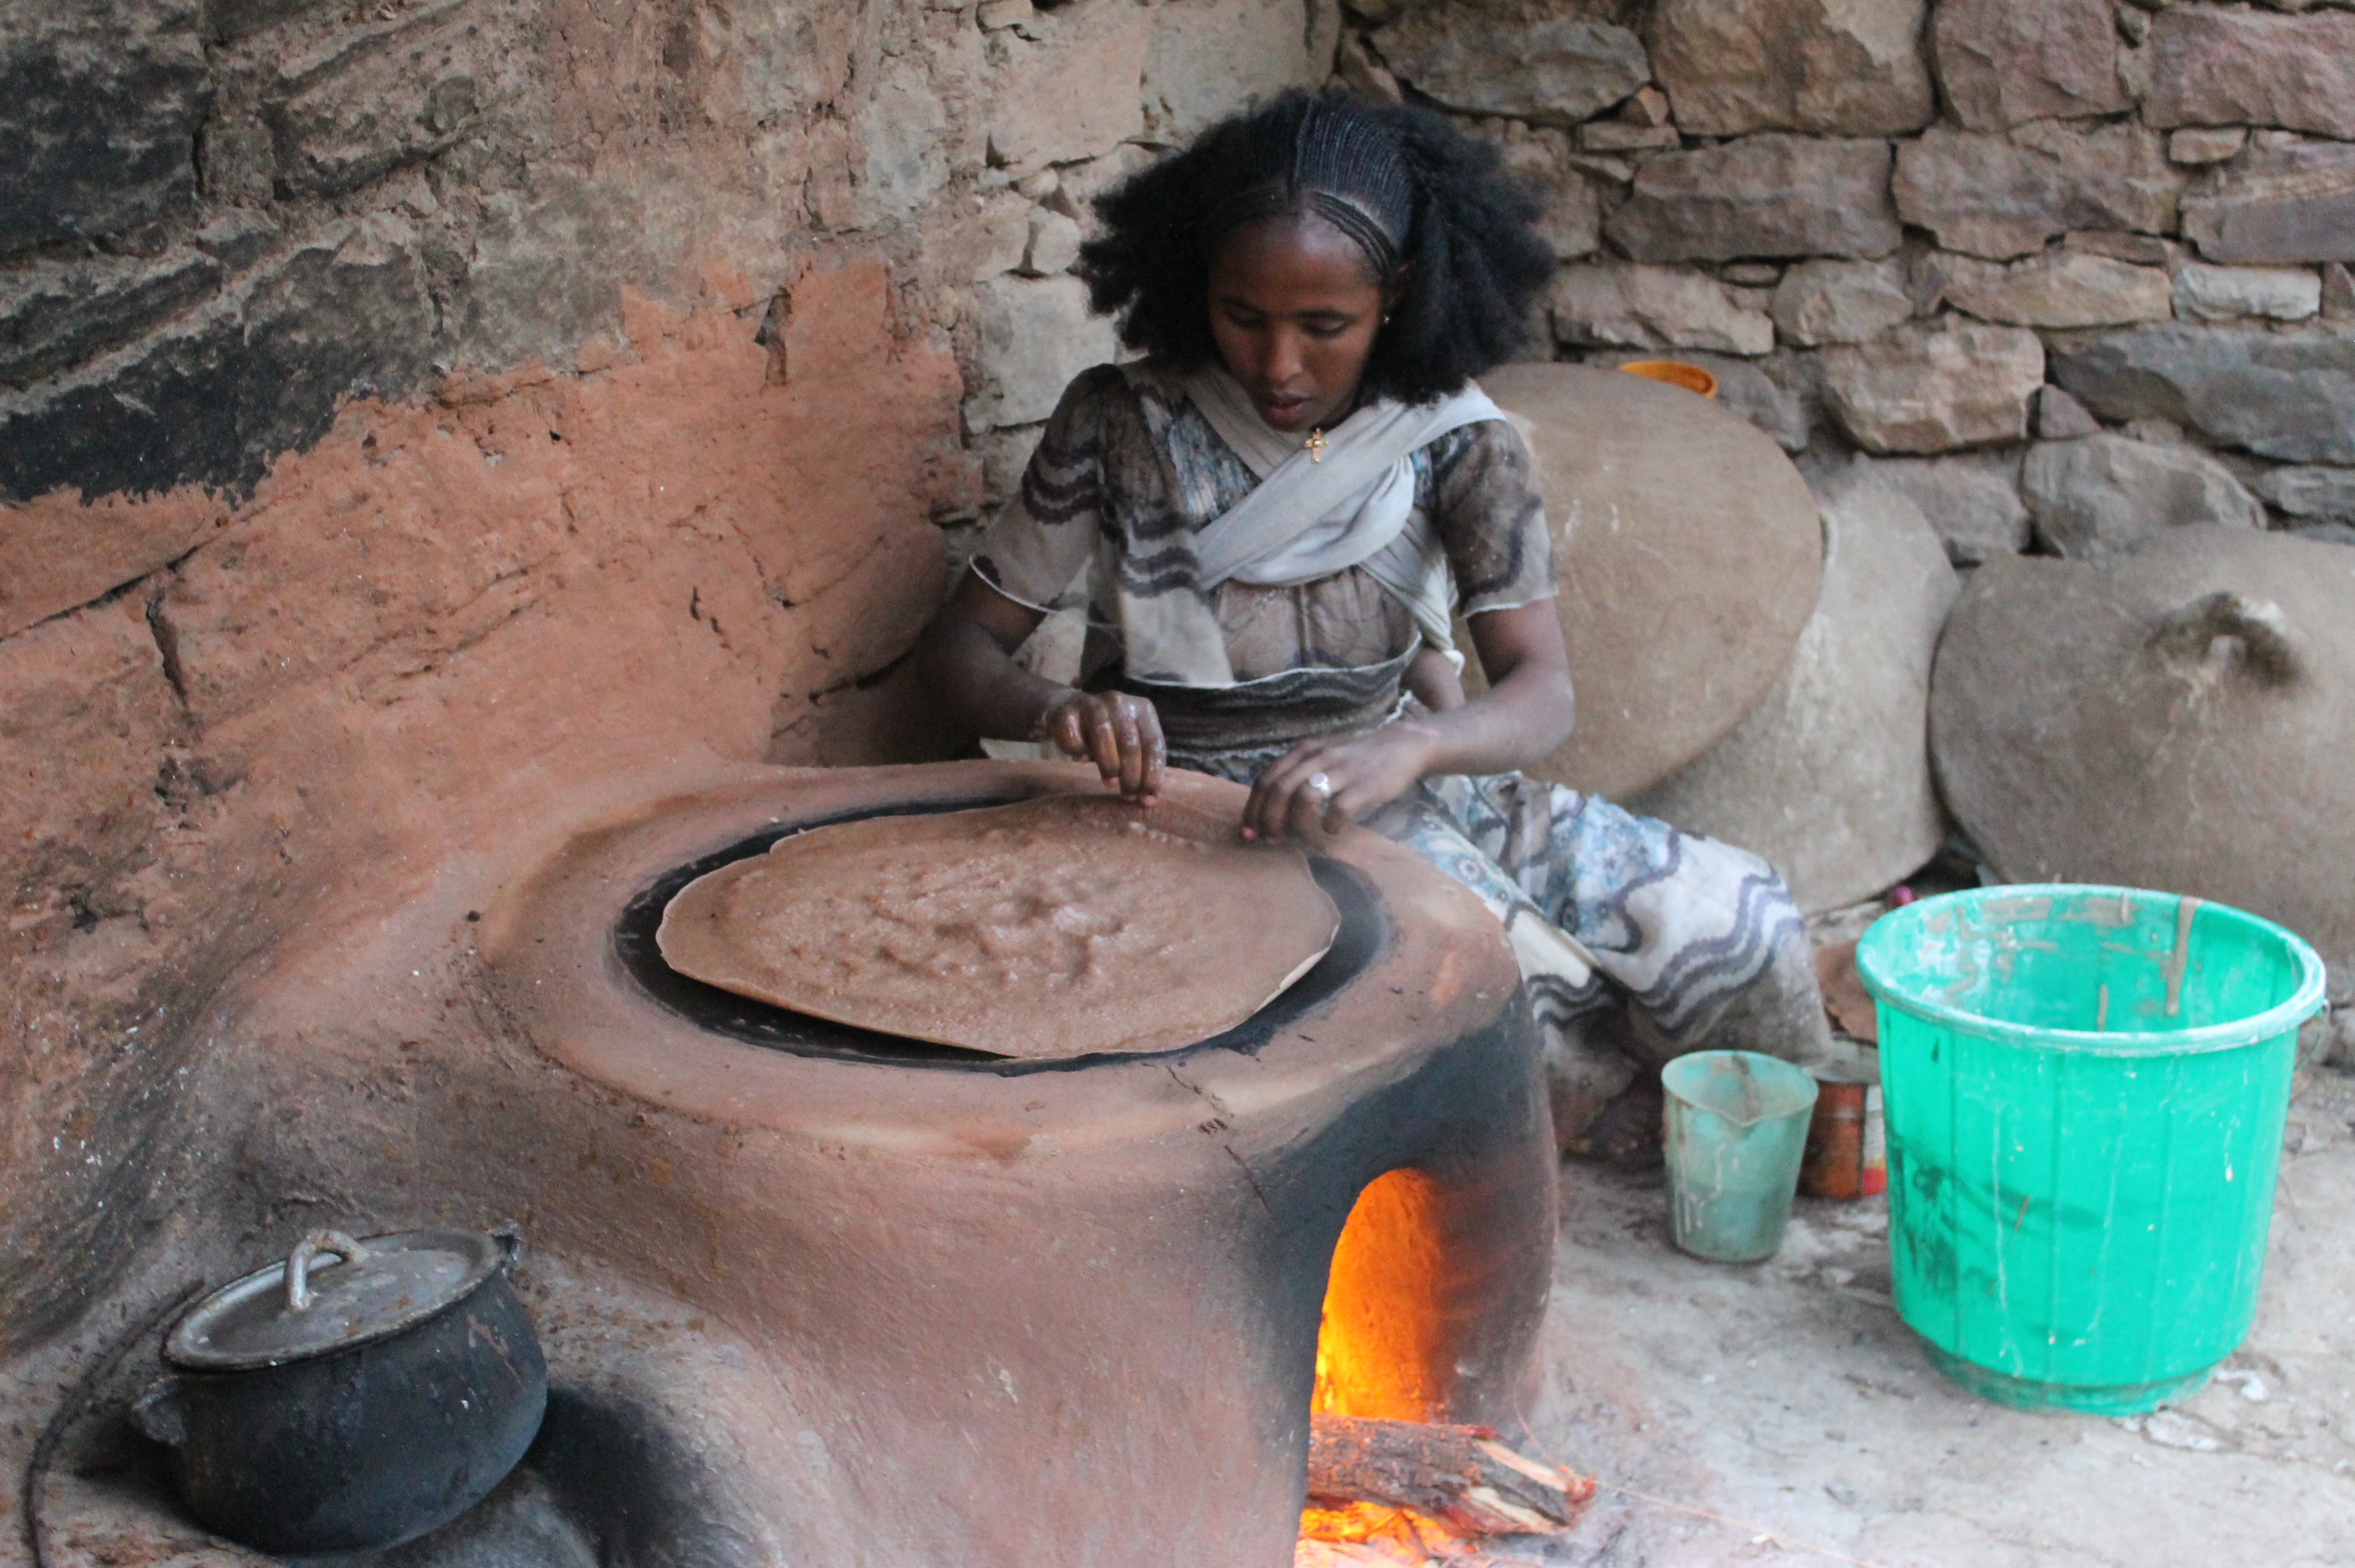
\includegraphics[width=1.0\textwidth]{ethiopian-woman-checking-bread}
  \caption[Ethiopian \emph{injera}]{An Ethiopian woman baking an \emph{injera}
      made using teff flour.  The image has been provided by Charliefleurene
      via Wikipedia.}
\end{center}
\end{figure}

If you used the flatbread option with less water, look at the size increase
of your dough. It should have increased at least \qty{50}{\percent} in size.
Also look out for bubbles on the sides of your container.

When using the pancake recipe, look out for bubbles on the surface of your dough.
In both cases use your nose to check the scent of your dough. Depending
on your sourdough starter's microbiome your dough will have
dairy, fruity, alcoholic notes or vinegary, acetic notes. Relying
on the smell of your dough is the best way to judge whether your
dough is ready or not. Timings are not reliable as they
depend on your starter and the temperature. If your dough
is ready too soon, you can now move it directly to the fridge and bake
it at a later, more convenient time. The low temperature will halt the fermentation
process\footnote{There are some exceptions. In some rare cases your starter
might also work at lower temperatures. You might have cultivated microbes that work best at
low temperatures. Nevertheless, fermentation
is always slower the colder it gets. A fridge really helps to preserve the state
of your dough.}
and your dough will last for several days. The longer you wait, the more sour the
bread is going to be. The fridge is a great option in case you want to
take the dough with you when visiting friends. People are going
to love you for the freshly baked flatbreads or pancakes. If you dare,
you can also taste a little bit of your raw uncooked dough. It is likely
going to taste relatively sour. I~do this frequently to better evaluate the
state of my doughs.

\begin{figure}[!htb]
\begin{center}
  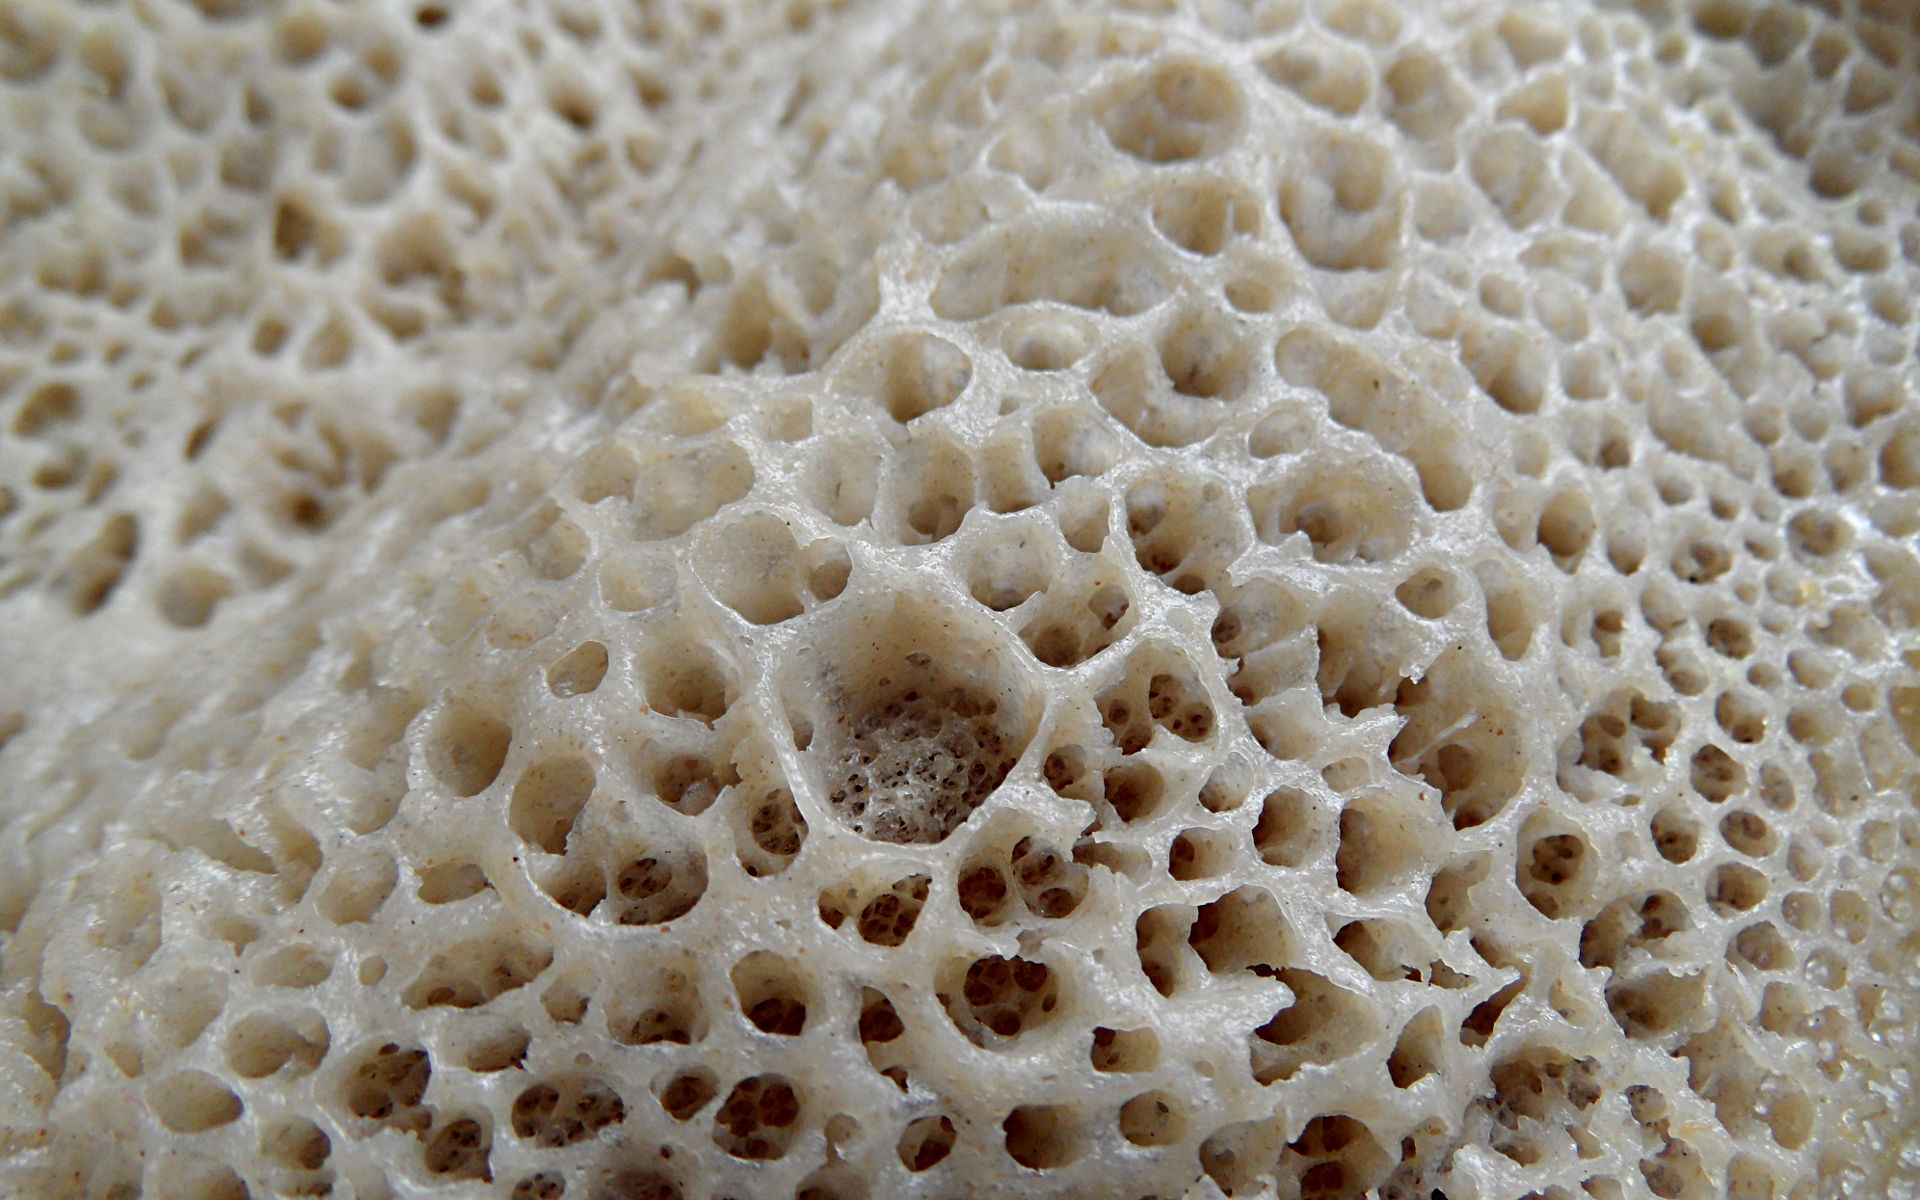
\includegraphics[width=1.0\textwidth]{injera-pancake-texture.jpg}
  \caption[Teff sourdough pancake]{A sourdough pancake made with teff flour.
      The pockets come from evaporated water and \ch{CO2} created by the
      microbes.  The image has been provided by Łukasz Nowak via Wikipedia.}
\end{center}
\end{figure}

If you are feeling lazy or don't have time, you could also use older sourdough starter
to make the dough directly without any prior starter feedings. Your sourdough starter
is going to regrow inside your dough. Remember that the
final bread might be a bit more on the sour side as the balance of yeast to
bacteria could be off. In the Table~\ref{tab:flat-bread-ingredients}
I~recommended using around \qtyrange{5}{20}{\percent}
of sourdough starter based on the flour to make the dough. If you were to follow
this approach, just use around \qty{1}{\percent} and make the dough directly.
The dough is probably going to be ready 24~hours later, depending on the temperature.

If you want to make sweet pancakes, add some sugar and optional eggs to your dough
now. A good quantity of eggs is around one~egg per \qty{100}{\gram} of flour.
Stir your dough a little bit and it will be ready to be used. You'll
have delicious sweet savory pancakes, the perfect combination. By
adding the sugar now, you make sure that the microbes don't have
enough time to fully ferment it. If you had added the sugar
earlier, no sweet flavor would be left  12~hours later.

To bake your dough heat your stove to medium temperature. Add a little bit of
oil to the pan. This helps with heat distribution and ensures even cooking.
With a spatula or a spoon place your dough in the pan. If your dough
was sitting in the fridge, bake it directly. There is no need to wait for your
dough to come to room temperature. If you have a lid,
place it on your pan. The lid helps to cook your dough from the top.
The evaporating water will circulate and heat up the dough's surface. When
making a flatbread, make the dough around \qty{1}{\cm} thick. When using the
pancake option, opt for around \qtyrange{0.1}{0.5}{\cm} depending on what you
like.

\begin{figure}[htb]
\begin{center}
  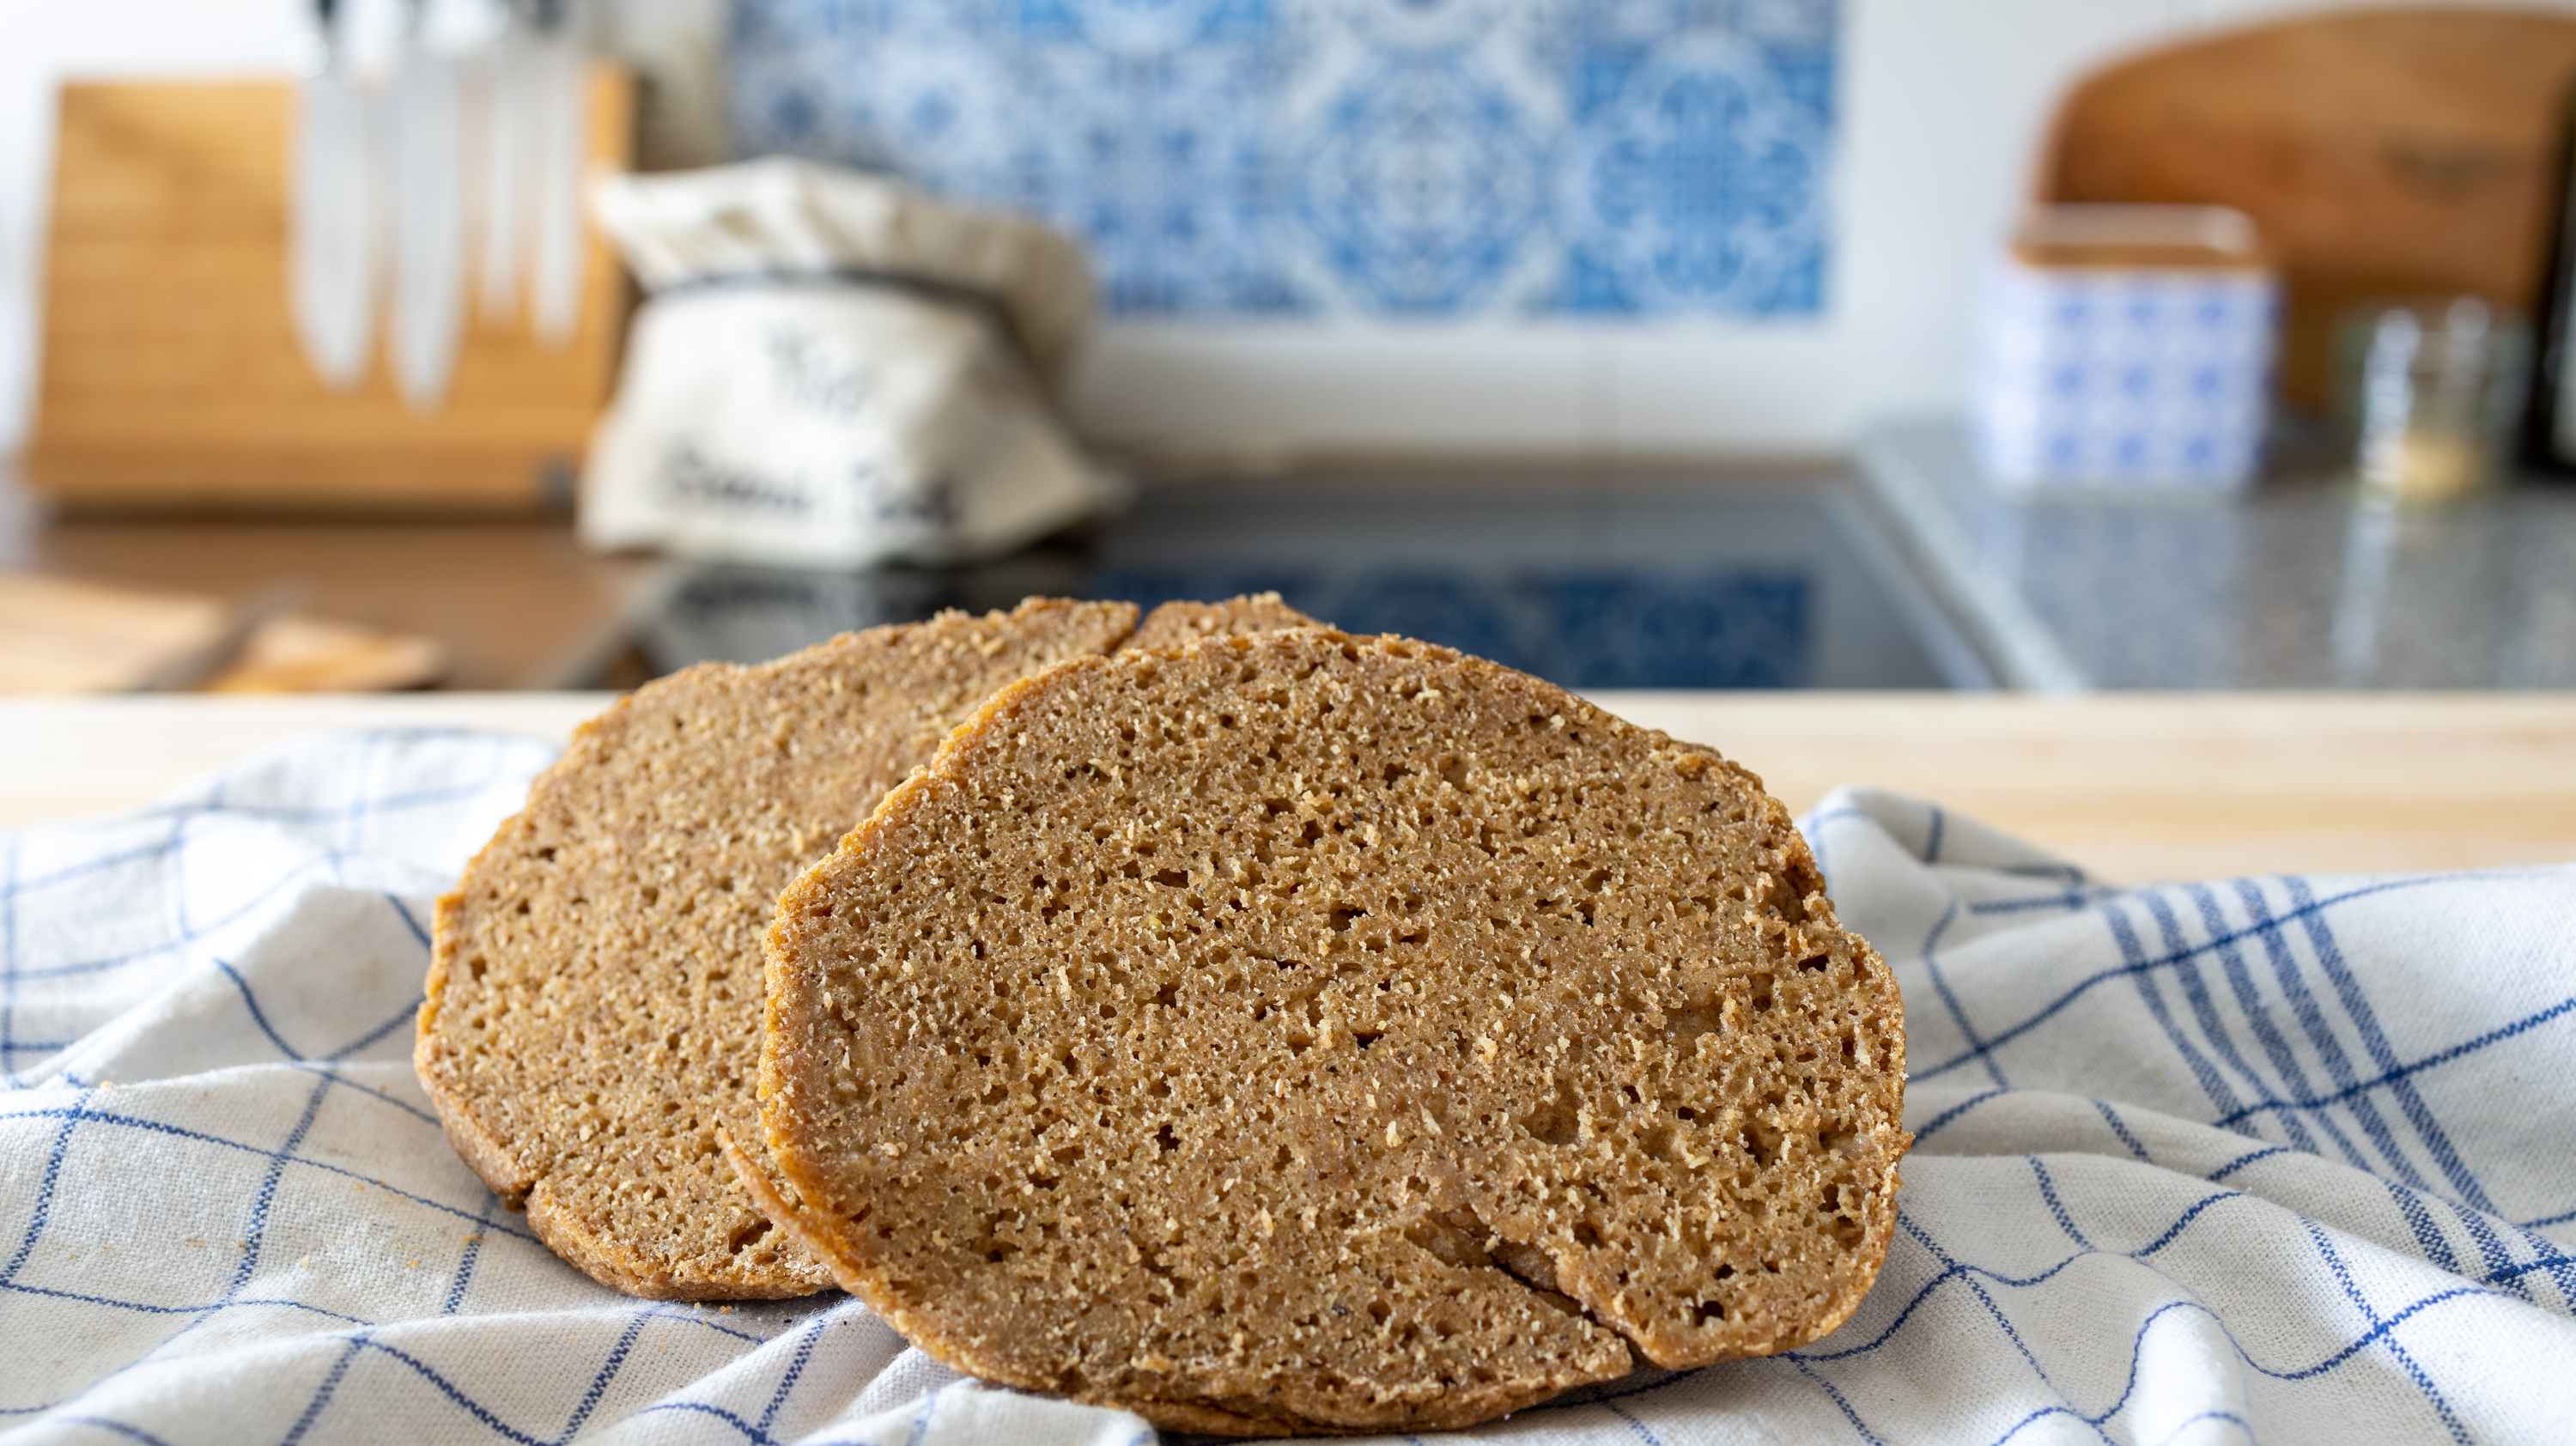
\includegraphics[width=1.0\textwidth]{einkorn-crumb.jpg}
  \caption[Einkorn crum]{The crumb of a flatbread made with einkorn as flour.
      Einkorn is very low in gluten and thus does not trap as much \ch{CO2} as
      a wheat based dough. To make the dough fluffier use more water or
      consider adding more wheat to the mix of your dough.}
\end{center}
\end{figure}

After 2--4~minutes flip over the pancake or flatbread. Bake it for the same
time from the other side. Depending on what you like, you can wait a little
longer to allow the bread to become a bit charred. The longer you
bake your bread, the more of the acidity is going to evaporate. If your
dough is a bit more on the sour side, you can use this trick to balance
out the acidity. This really depends on which flavor you are looking for.

When making a flatbread I~recommend wrapping the baked flatbreads in a kitchen
towel. This way more of the evaporating humidity stays inside of your bread,
making sure your flatbreads stay nice and fluffy for a longer period after the
bake. A similar strategy is used when making corn tortillas.

You can safely store the baked flatbreads or pancakes in your fridge
for weeks. When storing make sure to store them in an airtight plastic bag so that
they do not dry out. If they dry out, spray them with some water and toast them.
They will be almost as good as when they were freshly baked.

Keep a little bit of your unbaked dough. You can use it to make the next
batch of bread or pancakes for the next day. If you want to bake a few days later, add
a little bit of water and flour and store this mixture in your fridge
for as long as you like\footnote{The starter will stay good for months. If you expect to
leave it longer, consider drying a little bit of your sourdough starter.}.

\subsection{Simple flatbread recipe}%
\label{subsec:flat-bread-recipe}

By following the steps outlined in this section,
you'll be introduced to a versatile bread that's perfect for a myriad of
culinary applications. Whether you're scooping up a savory dip,
wrapping a flavorful filling, or simply enjoying a piece with a drizzle
of olive oil, these flatbreads are sure to impress.

\subsubsection*{Ingredients}

\begin{tabular}{r@{}rl@{}}
\qty{400}{\gram} &~(\qty{100}{\percent}) & Flour (wheat, rye, corn, whatever you have at hand)\\
\qty{320}{\gram} &  (\qty{80}{\percent}) & Water, preferably at room temperature\\
\qty{80}{\gram}  &  (\qty{20}{\percent}) & Active sourdough starter\\
\qty{8}{\gram}   &   (\qty{2}{\percent}) & Salt\\
\end{tabular}

\subsubsection*{Instructions}
\begin{description}
\item[Prepare the dough] In a large mixing bowl, combine the flour and water.
Mix until you have a shaggy dough with no dry spots.

Add the sourdough starter and salt to the mixture. Incorporate them thoroughly
until you achieve a smooth and homogenized dough.

\item[Fermentation:] Cover the bowl with a lid or plastic wrap. Allow the dough
    to rest and ferment until it has increased by at least \qty{50}{\percent}
    in size.  Depending on the temperature and activity of your starter, this
    can take anywhere from 4 to 24~hours.

\item[Cooking preparation:] Once the dough has risen, heat a pan over medium heat.
Lightly oil the pan, ensuring to wipe away any excess oil with a paper towel.

\item[Shaping and cooking:] With a ladle or your hands, scoop out a portion of
the dough and place it onto the hot pan, spreading it gently like a pancake.

Cover the pan with a lid. This traps the steam and ensures even cooking
from the top, allowing for easier flipping later.

After about 5~minutes, or when the bottom of the flatbread has a
golden-brown crust, carefully flip it using a spatula.

\emph{Adjusting cook time.} If the flatbread appears too dark,
remember to reduce the cooking time slightly for the next one.
Conversely, if it's too pale, allow it to cook a bit longer before flipping.

Cook the flipped side for an additional 5~minutes or until it's also golden
brown.

\item[Storing:] Once cooked, remove the flatbread from the pan and place it on a
kitchen towel. Wrapping the breads in the towel will help retain their
softness and prevent them from becoming overly crisp.
Repeat the cooking process for the remaining dough.

\item[Serving suggestion:] Enjoy your sourdough flatbreads warm,
paired with your favorite dips, spreads, or as a side to any meal.

\end{description}
\section{Loaf pan bread}

Loaf pan bread is made using the help of a special loaf pan
or loaf tin. The edges of the pan provide additional support
for the dough to rise. Making a bread using a loaf pan requires
an oven.

\begin{figure}[!htb]
  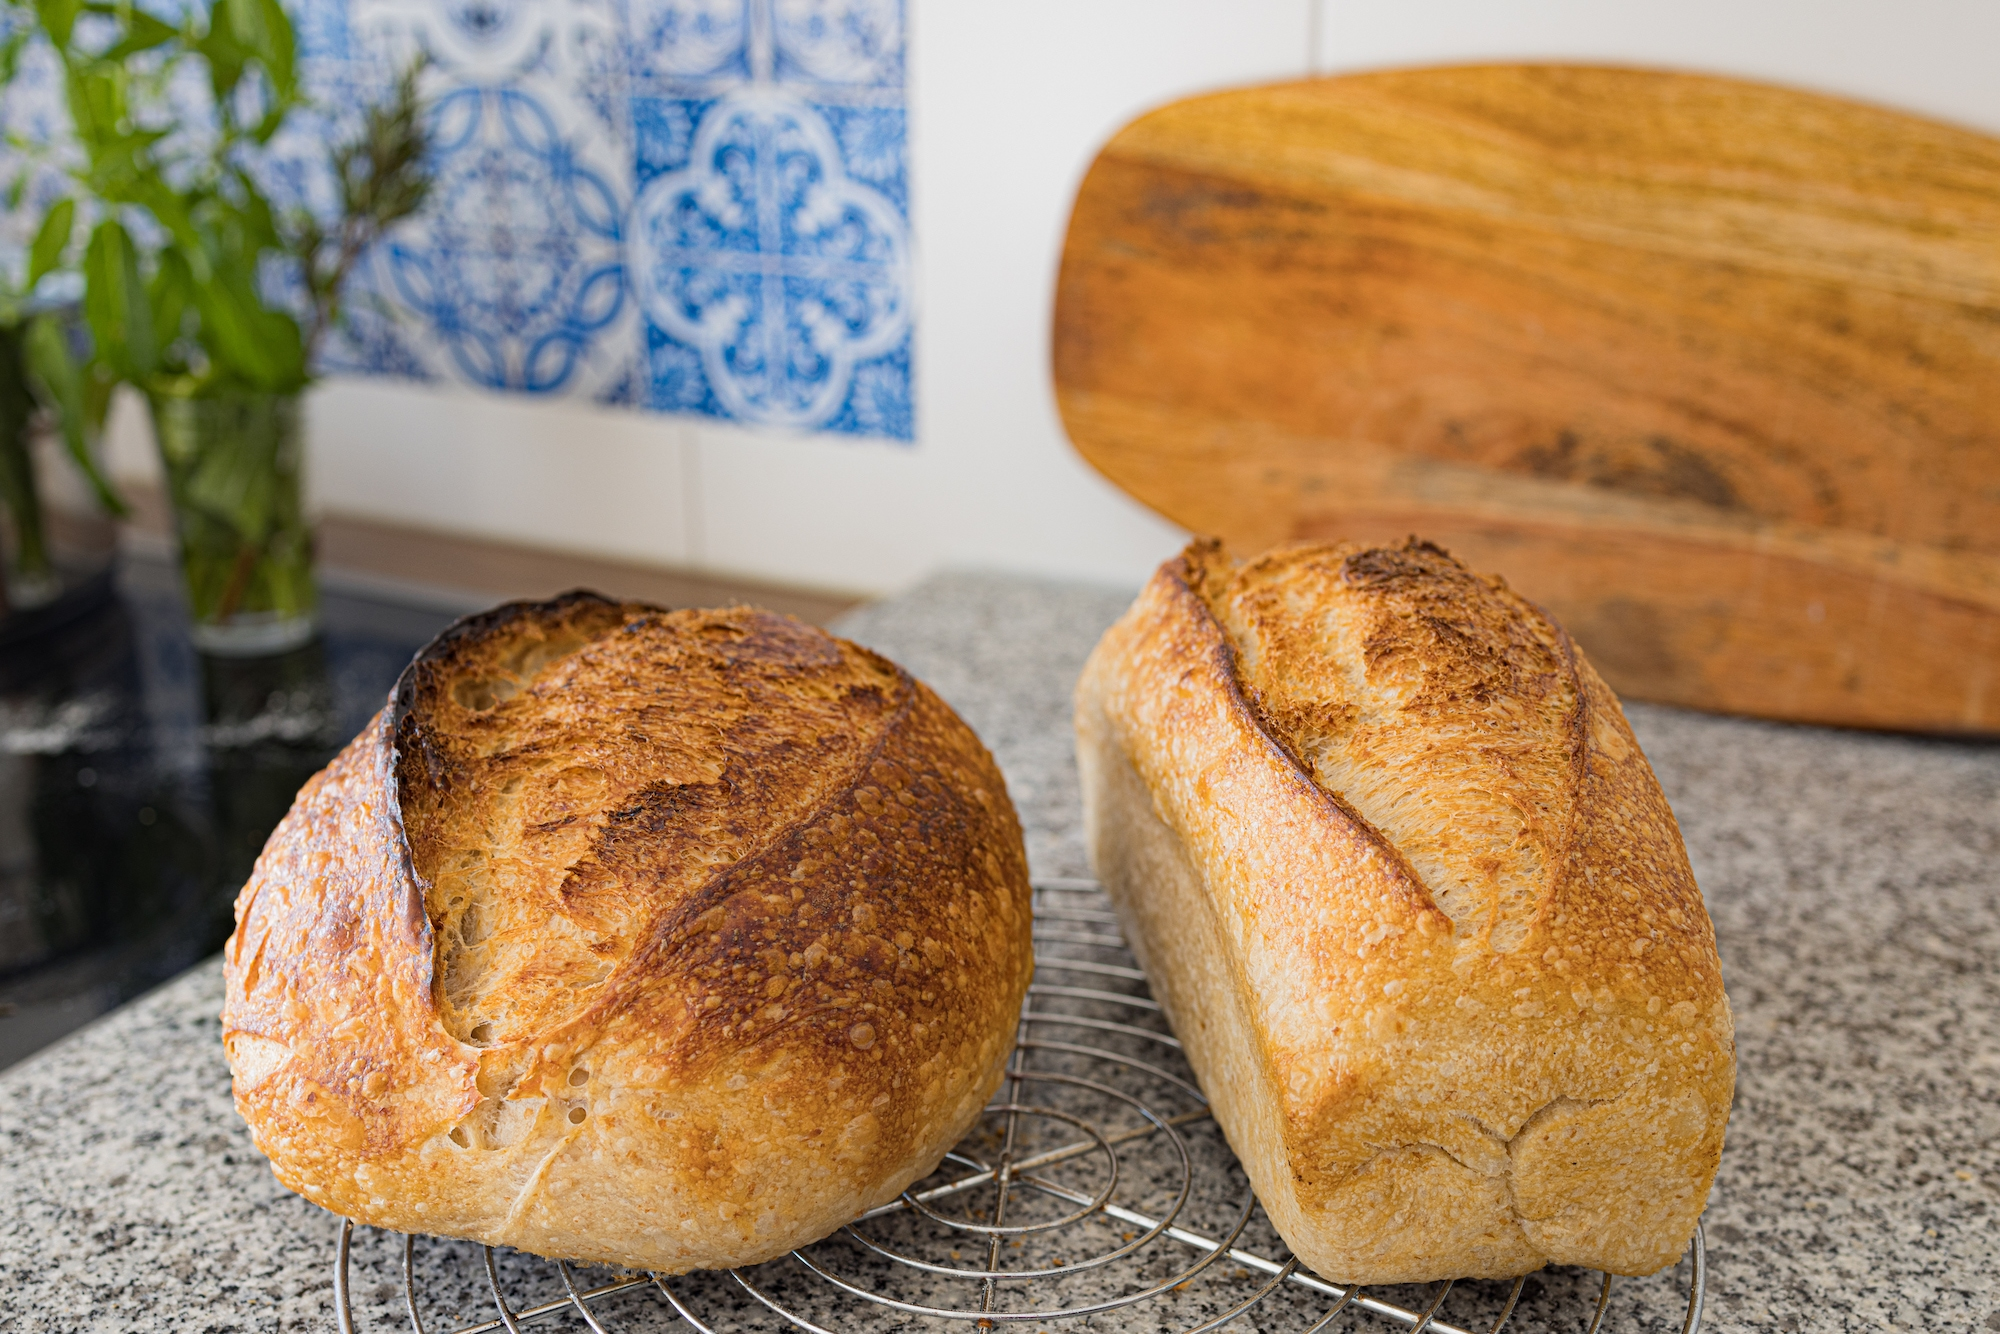
\includegraphics[width=\textwidth]{loaf-pan-free-standing.jpg}
  \caption[Freestanding bread and pan bread]{A freestanding bread and a wheat
      loaf pan bread. Both of them received a small incision before baking
      which helps to control how they open up.}%
  \label{fig:free-standing-loaf-pan}
\end{figure}

After mixing your dough, you can place it directly into the loaf pan.
This makes the whole process simpler since you can skip steps such
as shaping the dough.

To make a great loaf pan bread with little work:

\begin{enumerate}
    \item Mix the ingredients of your dough (gluten free works too)
    \item Place into the loaf pan
    \item Wait until your dough has roughly doubled in size
    \item Bake in a non pre-heated oven for around 30--50~minutes
\end{enumerate}

Knowing the exact baking time is sometimes a little challenging
as it might be that the outside of your bread is cooked but
the inside is still raw. The best way is to use a thermometer
and measure the core temperature. At around  \qty{92}{\degreeCelsius}
(\qty{197}{\degF}) your dough is done. I~generally bake loaf pan bread at
around  \qty{200}{\degreeCelsius} (\qty{390}{\degF}), which is a little less
than my freestanding bread which I~bake at  \qty{230}{\degreeCelsius}
(\qty{445}{\degF}). That's because it takes a while for the dough
to bake properly inside the loaf pan. The edges don't heat up
as quickly. Then the top part of the dough is properly cooked, while
the inside isn't yet. When baking make sure to use steam
or simply place another equally sized loaf pan on top
of your loaf pan. This way you simulate a Dutch oven. The dough's
evaporating moisture will stay inside.

A good trick to make excellent loaf pan bread is to make a very
sticky dough. You can opt for a hydration of \qtyrange{90}{100}{\percent}, almost
resembling a default sourdough starter. Just like with flatbread,
the high humidity helps to make a more airy, fluffy crumb. The bread will
also be a bit chewier. This type of bread made with rye is my family's favorite
style of bread.  The hearty rye flavor paired with the sticky consistency really
makes an excellent sandwich bread.

To improve the structure you can also consider using around \qty{50}{\percent}
wheat flour in your mix. The gluten network will develop as your
dough ferments and allow for more gas to be trapped in the dough.

A common problem you will face when making a loaf pan bread is
the dough sticking to the pan. Use a generous amount of oil to grease
your pan. A nonstick vegetable oil spray can do wonders.
Don't clean your loaf pans with soap. Just use a kitchen towel
to clean them. With each bake a better patina forms, making your
pan more and more stick resistant.

What's amazing about this type of bread is that it works
with every flour. The overall time to work the dough is probably
less than 5~minutes, making it very easy to integrate
into your daily routine. Furthermore, loaf pans use the space
in your oven very efficiently. Using pans I~can
easily bake 5 loaves at the same time in my home oven.
Normally I~would need multiple baking sessions for
freestanding loaves.

\section{Free standing bread}

A freestanding loaf is baked entirely without supporting
baking vessels in your oven. To make a freestanding loaf more steps
and tools are required.

\begin{figure}[!htb]
\begin{center}
  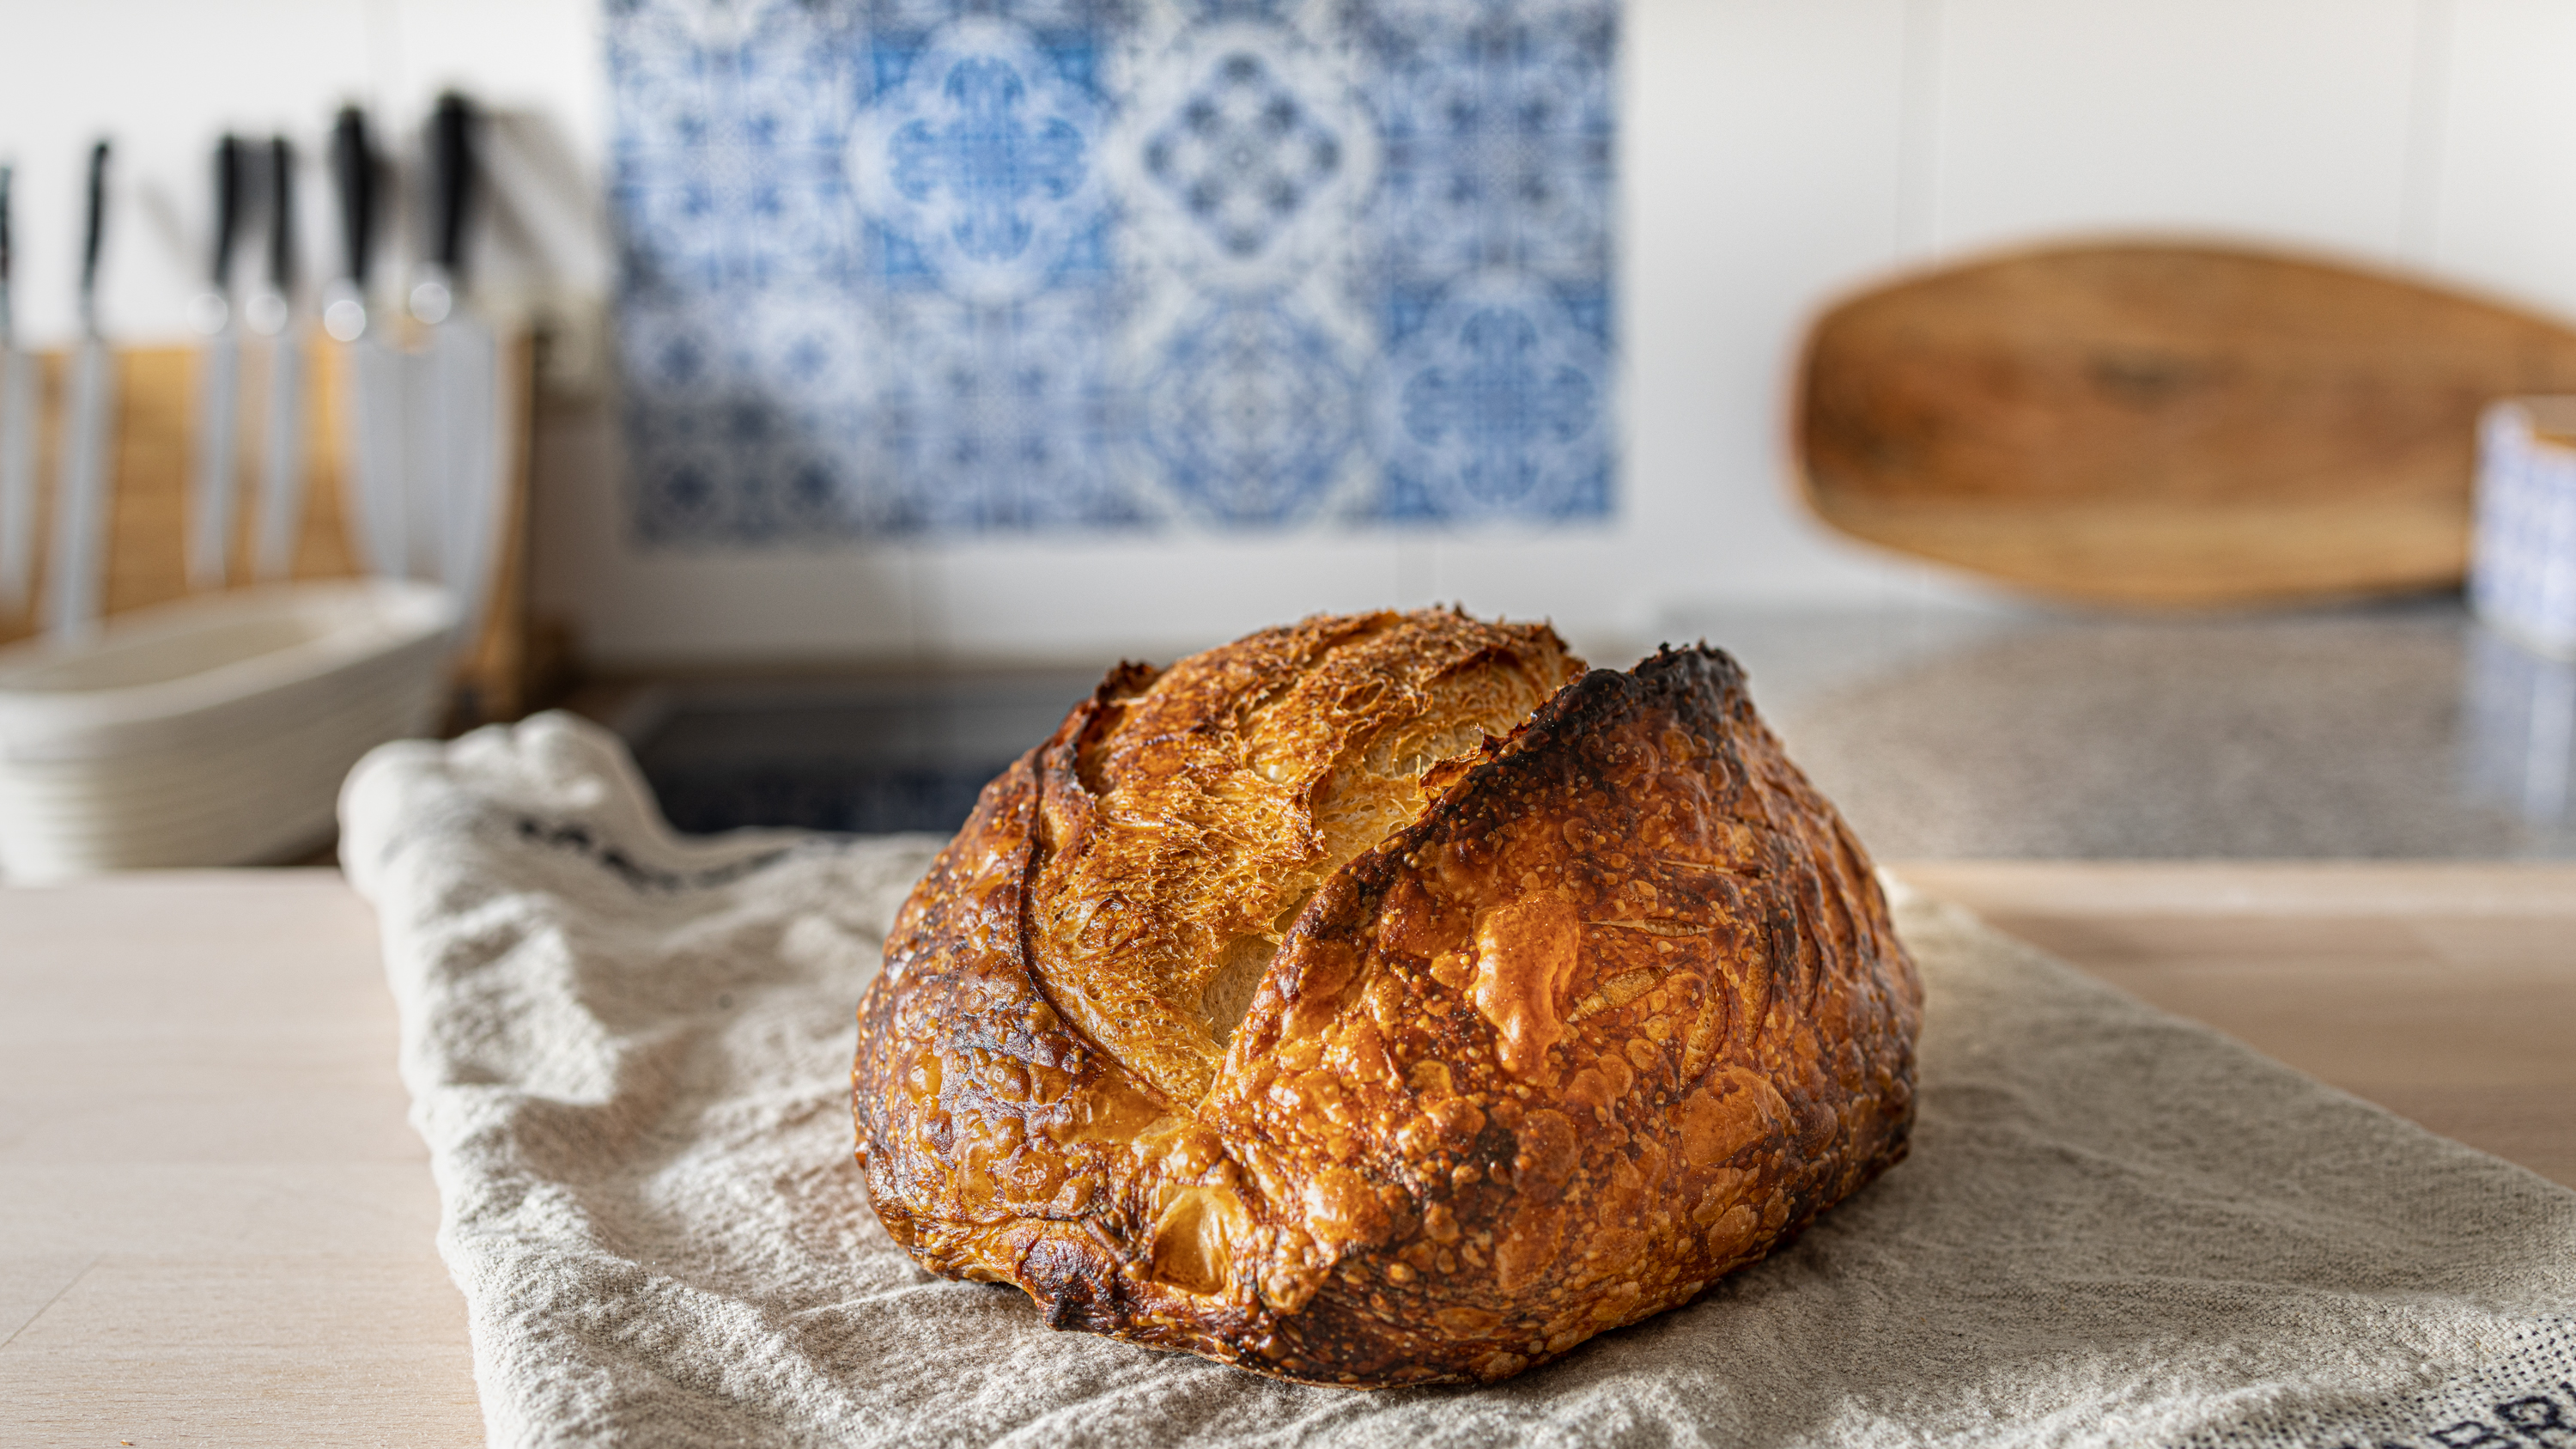
\includegraphics[width=1.0\textwidth]{free-standing-loaf.jpg}
  \caption[Freestanding sourdough bread]{A freestanding sourdough bread. Note
      the incision known as an \emph{ear} and the oven spring clearly
      distinguish this type of bread from flatbread and loaf pan bread.}
\end{center}
\end{figure}

When using wheat, make sure to mix your dough enough to develop a gluten network.
Allow the dough to reach a certain size increase during the fermentation.
Afterward, divide and pre-shape the dough into the desired visual shape you
would like. Each shape requires a different technique. Sometimes achieving
the right shape can be challenging. Making a baguette, for instance,
requires performing more steps. Mastering this technique takes several attempts.

Once the dough is shaped, it is proofed again for a certain
period of time. Once the dough is ready, a sharp tool such
as a razor blade is used to make an incision into the dough.
This helps control how the dough opens up during the baking process.

All these steps require practice. Each of them has to be
performed perfectly, without mistakes.
But after baking you will be rewarded with a beautiful bread
with great taste and consistency.

There is a dedicated recipe and tutorial for this type of bread in the
\nameref{chapter:wheat-sourdough} chapter.
